\documentclass[12pt,a4paper]{article} 
\usepackage{tikz}
\usepackage{float}
\usepackage{graphicx}
\usepackage{multirow}
\usepackage{setspace} 
\usepackage{graphicx}
\usepackage{times}
\pagenumbering{roman}
\usepackage{geometry}

\geometry{verbose,tmargin=2cm,bmargin=2cm,lmargin=3cm,rmargin=2cm}
\usepackage{fancyhdr} 
%\linespread{1.05} 
\usepackage{tikz}
\usetikzlibrary{arrows}
\usetikzlibrary{shapes.geometric}

\tikzstyle{kres} = [rectangle, rounded corners, minimum width=1cm, minimum height=0.5cm,text centered, draw=black]
\tikzstyle{nad} = [trapezium, trapezium left angle=60, trapezium right angle=100, minimum width=1cm, minimum height=0.5cm, text centered, draw=black]
\tikzstyle{sim} = [trapezium, trapezium left angle=60, trapezium right angle=100, minimum width=1cm, minimum height=0.5cm, text centered, draw=black]
\tikzstyle{garis} = [thick,->,>=stealth]
\usetikzlibrary{shapes,arrows}

\begin{document} % Mulai Penulisan Laporan
\onehalfspacing
\begin{titlepage}

\title{\textbf{LAPORAN PRAKTIKUM ELEKTRONIKA DASAR
\\ OP-AMP DIFFERENTIATOR,INTEGRATOR,ADDER DAN SUBTRACTOR}}  %Judul Laporan
%\title{\textbf{FOTOKATALISIS}}  %Judul Laporan
\author{\textbf {Dosen : Mada Sanjaya WS, Ph.D  }
\\ \textbf{Asisten Lab : Noer Ardiansyah Laksana (1177030025)}
\\ \textbf{ }
\\ \textbf{Disusun Oleh :}
\\ \textbf{Muhamad Fahmi Adzkar} \textbf {(1187030024)}
\\ \textbf{Kelompok 3 :}
\\ \textbf{Hani Hikmawati} \textbf {(1187030014)}
\\ \textbf{Sri Rahayu} \textbf {(1187030036)}
\\ \textbf{Yuni Rahayu} \textbf {(1187030041)}}

\maketitle
\begin{center}
\vspace{1cm}

\includegraphics[width=4cm]{uin.png}
\vspace{1cm}

JURUSAN FISIKA\\
FAKULTAS SAINS DAN TEKNOLOGI\\
UIN SUNAN GUNUNG DJATI BANDUNG\\
2019\\
\end{center}
\end{titlepage}

\renewcommand\abstractname{Abstract} %Untuk Abstrak Bahasa Inggris
\begin{abstract} %Untuk Abstrak Bahasa Inggris
Experiments have been conducted on the Op-Amp Adder and Op-Amp Subtractor in the Advanced Physics Laboratory UIN Bandung with the aim of understanding the series of Adder and Subtractor, analyzing the working principle of the series of Adder and Subtractor, knowing the input and output waves in each circuit, and can calculate the output voltage in each circuit. From the result of the practicum, it was found that the output voltage 1 and the input 2 had a sense difference of 180 degrees in the waveform. The amount of output in the Op-Amp subtractor is a reduction of the input signal 1 and the input signal 2 and does not have a difference in taste so that the waveform is in tandem.

\textit{Keywords: Op-Amp, Adder, Subtractor}
\end{abstract}

\begin{abstract}
Telah dilakukan percobaan tentang Op-Amp Adder dan Op-Amp Subtractor di Laborstorium Advance Physics UIN bandung yang bertujuan untuk memahami rangkaian adder dan subtractor, menganalisa prinsip kerja rangkaian adder dan subtractor, mengetahui gelombang input dan output pada setiap rangkaian, dan menghitung tegangan output dari setiap rangkaian. Dari hasil praktikum, diperoleh bahwa besarnya tegangan output pada Op-Amp adder merupakan penjumlahan dari sinyal input 1 dan sinyal input 2 serta memiliki beda fasa sebesar 180 derajat pada bentuk gelombangnya. Besarnya tegangan output pada Op-Amp Subtractor merupakan pengurangan dari sinyal input 1 dan sinyal input 2 serta tidak memiliki beda fasa sehingga bentuk gelombangnya beriringan. 

\textit{Kata Kunci: Op-Amp, Adder, Subtractor }
\end{abstract}


\newpage
\section{PENDAHULUAN}
\paragraph{1.1 Latar Belakang}
\subparagraph{ }
	Penguat Operasional (Operasional Amplifier) atau yang biasa disebut Op-Amp merupakan suatu jenis penguat elektronika dengan hambatan (coupling) arus searah yang memiliki faktor penguatan sangat besar dengan dua masukan dan satu pengeluaran.
\subparagraph{ }
	Pada umumnya penguat operasional tersedia dalam bentuk sirkuit terpadu dan yang paling banyak digunakan adalah ranfkaian seri. Penguat opersional dalam rangkaian terpadu memiliki karakteristik yang mendekati karakteristik penguat operasional ideal tanpa perlu memperhatikan apa yang terdapat di dalamnya.
\subparagraph{ }
Penguat operasional adalah perangkat yang sangat efisien dan serba guna. Contoh penggunaan penguat operasional adalah untuk operasi matematika sederhana seperti penjumlahan dan pengurangan terhadap tegangan listrik hingga dikembangkan kepada penggunaan aplikatif seperti komparator dan osilator dengan distorsi rendah serta pengembangan alat komunikasi. Selain itu, aplikasi pemakaian op-amp juga meliputi bidang elektronika audio, pengatur tegangan DC, tapis aktif, penyearah presisi, pengubah analog digital dan pengubah digital ke analog, pengolah isyarat seperti cuplik tahan, penguat pengunci, kendali otomatik, computer analog, elektronika nuklir, dan lain-lain.

\paragraph{1.2 Tujuan}
\subparagraph{ }
Adapun tujuan dilakukannya praktikum ini yaitu:
\begin{enumerate}
\item Mampu memahami rangkaian adder dan subtractor.
\item Mampu menganalisa prinsip kerja rangkaian adder dan subtractor.
\item Mengetahui gelombang input dan output pada setiap rangkaian.
\item Dapat menghitung tegangan output dari setiap rangkaian.
\end{enumerate}


\newpage
\section{Landasan Teori}
\subsection{Dasar Teori}
\paragraph{ }
\textbf{1.Penguat operasional}
\subparagraph{ }
 Penguat operasional (bahasa Inggris: operational amplifier) atau yang biasa disebut op-amp merupakan suatu jenis penguat elektronika dengan sambatan (bahasa Inggris: coupling) arus searah yang memiliki bati (faktor penguatan atau dalam bahasa Inggris: gain) sangat besar dengan dua masukan dan satu keluaran.Penguat operasional pada umumnya tersedia dalam bentuk sirkuit terpadu dan yang paling banyak digunakan adalah seri 741.

Penguat operasional adalah perangkat yang sangat efisien dan serba guna.Contoh penggunaan penguat operasional adalah untuk operasi matematika sederhana seperti penjumlahan dan pengurangan terhadap tegangan listrik hingga dikembangkan kepada penggunaan aplikatif seperti komparator dan osilator dengan distorsi rendah.

Penguat operasional dalam bentuk rangkaian terpadu memiliki karakteristik yang mendekati karakteristik penguat operasional ideal tanpa perlu memperhatikan apa yang terdapat di dalamnya.Karakteristik penguat operasional ideal adalah:
\begin{enumerate}
\item Bati tegangan tidak terbatas.
\item Impedansi masukan tidak terbatas.
\item Impedansi keluaran nol.
\item Lebar pita tidak terbatas.
\item Tegangan offset nol (kondisi ketika masukan sebesar nol).
\end{enumerate}
	
\begin{flushright}
(Wikipedia.com)
\end{flushright}

\subparagraph{ }
\textbf{2.Rangkaian ADDER (penjumlahan)}
\subparagraph{ }
 Adder merupakan rangkain ALU (Arithmetic and Logic Unit) yang digunakan untuk menjumlahkan bilangan. Karena adder digunakan untuk memproses operasi aritmatika, maka adder juga sering disebut rangkaian kombinasional aritmatika. Ada 3 jenis Adder, yaitu:
Rangkaian adder yang hanya menjumlahkan dua bit disebut Half Adder.
Rangkaian adder yang hanya menjumlahkan tiga bit disebut Full Adder.
Rangkaian adder yang menjumlahkan banyak bit disebut Paralel Adder.
\subparagraph{ }
1. Half Adder.
Rangkain half adder merupakan dasar bilangan biner yang masing-masing hanya terdiri dari satu bit, oleh karena itu dinamakan penjumlah tak lengkap.
Jika A=0 dan B=0 dijumlahkan, hasilnya S (Sum) = 0.
Jika A=0 dan B=0 dijumlahkan, hasilnya S (Sum) = 1.
Jika A=1 dan B=1 dijumlahkan, hasilnya S (Sum) = 0. Dengan nilai pindahan Cy (Carry Out) = 1.
Dengan demikian, half adder memiliki dua masukan (A dan B), dan dua keluaran (S dan Cy). 

Dari tabel diatas, terlihat bahwa nilai logika dari Sum sama dengan nilai logika dari gerbang XOR, sedangkan nilai logika Cy sama dengan gerbang logika  AND. Dari tabel diatas, dapat dibuat rangkaian half adder seperti dibawah ini.

\subparagraph{ }
2. Full Adder
Full adder adalag mengolah data penjumlahan 3 bit bilangan atau lebih (bit tidak terbatas), oleh karena itu dinamakan rangkaian penjumlah lengkap. Perhatikan tabel dibawah ini.

\subparagraph{ }
3. Paralel Adder
Paralel Adder adalah rangkaian Full Adder yang disusun secara paralel dan berfungsi untuk menjumlahkan bilangan biner berapa pun bitnya, tergantung jumlah Full Adder yang diparalelkan. Gambar dibawah ini menunjukan Paralel Adder yang terdiri dari 4 buah Full Adder yang disusun paralel sehingga membentuk sebuah penjumlahan 4 bit.

\begin{flushright}
(Wikipedia.com) 
\end{flushright}

\paragraph{ }
\textbf{3. Rangkaian Subtractor}
\subparagraph{ }
	Sama seperti rangkaian penjumlahan biner, pada rangkaian pengurangan biner juga dapat dibagi menjadi half subtactor dan full subtractor. Rangkaian half subtractor merupakan dasar untuk menyusun atau membuat rangkaian full subtractor. Jadi untuk dapat memahami rangkaian full subtraktor, kita wajib terlebih dahulu memahami prinsip dasar dari rangkaian half subtractor. Berikut ini adalah penjelasan dari rangkaian half subtractor dan full subtractor.

Rangkaian Half Subtractor
Rangkaian pengurang setengah atau half subtractor merupakan implementasi dari operasi pengurangan dasar dua bilangan biner. 

Pada rangkaian ini tidak ada pengurangan borrow in yang dilibatkan yang artinya pada rangkaian ini proses pengurangan belum sempurna. Berikut ini adalah rumus dasar pengurangan biner yang dapat dilakukan oleh half subtractor.

Rangkaian Full Subtractor
Ketidakmampuan rangkaian half subtractor dalam melibatkan borrow in dapat diatasi dengan menggunakan Rangkaian full subtractor. Sesuai dengan namanya full subtractor merupakan penjumlahan penuh yang maksudnya sudah melibatkan borrow out dan borrow in dalam prosesnya. Sehingga proses pengurangan dapat dilakukan dengan sempurna. 

Pada dasarnya rangkaian full subtractor ini dibentuk dari dua buah half subtractor yang masing-masing borrow outnya digabungkan dengan sebuah gerbang or. Adapun simbol dari rangkaian full subtractor ini dapat dilihat pada gambar berikut:
	
\begin{flushright}
(Wikipedia.com) 
\end{flushright}

\newpage
\section{METODE PRAKTIKUM}
\subsection{Waktu dan Tempat}
\paragraph{ }
Praktikum ini dilaksanakan pada:
\\ 		Tanggal : jum'at, 6 Desember 2019
\\ 		Waktu : 07.00 WIB - Selesai
\\ 		Tempat : Advance Physics 


\subsection{Alat dan Bahan}
Alat dan bahan yang digunakan dalam praktikum ini diantaranya adalah : 
\subparagraph*{ }
\begin{tabular}{|l|l|l|}  \hline
No & Alat dan Bahan  & Jumlah  \\ \hline
1  & Projek board & 1 Buah \\ \hline
2  & IC LM741 & satu set \\ \hline
3  & Baterai 9 volt & Secukupnya \\ \hline
4  & Kancing Baterai 3 Pin & 1 Buah \\ \hline
5  & Kabel Tunggal  & Secukupnya \\ \hline
6  & Resistor  & 2 Buah \\ \hline
7  & Multimeter & Satu set \\ \hline
8  & Osiloskop & Satu set \\ \hline
\end{tabular}

  
    
\subsection{Prosedur Percobaan}
\subparagraph{3.3.1 Percobaan Rangkaian ADDER }
\subparagraph{ }
\textbf{Rangkaian Inverting} Rangkaian disusun sesuai dengan gambar di lampiran dan project board. Kemudian siapkan alat dan bahan yang digunakan. Kemudian Susun rangkaian sesuai dengan gambar simulasi di papan tulis. kemudian ukur besar resistansi pada resistor. Dilanjut dengan diukurnya besar tegangan pada rangkaian inverting dan ketika diberikan tegangan sebesar 9 V arus DC, diukur  V pada rangkaian inverting ketika kondisi stabil di osiloskop. kemudian data ditulis pada tabel.
	
\subparagraph{3.3.2 Percobaan Rangkaian Subtractor }
\subparagraph{ }
	\textbf{Rangkaian Non-Inverting} Rangkaian disusun sesuai dengan gambar di lampiran dan project board. Kemudian siapkan alat dan bahan yang digunakan. Kemudian Susun rangkaian sesuai dengan gambar simulasi di papan tulis. kemudian ukur besar resistansi pada resistor. Dilanjut dengan diukurnya besar tegangan pada rangkaian inverting dan ketika diberikan tegangan sebesar 9 V arus DC, diukur  V pada rangkaian inverting ketika kondisi stabil di osiloskop. kemudian data ditulis pada tabel.

\subsection{Diagram Alir}
\subsubsection{Percobaan Rangkaian ADDER }
\tikzstyle{line} = [draw, -latex']
\tikzstyle{cloud} = [draw, rectangle,fill=blue!20, node distance=3cm,
    minimum height=0.7cm]
\tikzstyle{kres} = [draw, rectangle, rounded corners,fill=blue!20, node distance=3cm,
    minimum height=0.7cm]
\begin{tikzpicture}[node distance = 1.3cm, auto]
    % Place nodes
       \node [kres] (a) {Siapkan alat dan bahan yang digunakan};
       \node [cloud, below of = a , node distance = 1.5cm] (b) {Susun rangkaian sesuai dengan gambar};         
       \node [cloud, below of = b , node distance = 1.5cm] (c) {Mengukur nilai resistansi pada resistor};
       \node [cloud, below of = c , node distance = 1.5cm] (d) {Masukan tegangan Baterai 9 Volt DC};
       \node [cloud, below of = d , node distance = 1.5cm] (e) {Mengukur V output dengan osiloskop ketika kondisi gelombang stabil};        
       \node [cloud, below of = e , node distance = 1.5cm] (f) {Hasil data ditulis pada tabel};
        
        
     % Draw edges
    \path [line] (a) -- (b);
    \path [line] (b) -- (c);
    \path [line] (c) -- (d);
    \path [line] (d) -- (e);
    \path [line] (e) -- (f);
    \end{tikzpicture}   

	\subsubsection{Percobaan Rangkaian Subtractor }
\tikzstyle{line} = [draw, -latex']
\tikzstyle{cloud} = [draw, rectangle,fill=blue!20, node distance=3cm,
    minimum height=0.7cm]
\tikzstyle{kres} = [draw, rectangle, rounded corners,fill=blue!20, node distance=3cm,
    minimum height=0.7cm]
\begin{tikzpicture}[node distance = 1.3cm, auto]
    % Place nodes
       \node [kres] (a) {Siapkan alat dan bahan yang digunakan};
       \node [cloud, below of = a , node distance = 1.5cm] (b) {Susun rangkaian sesuai dengan gambar};         
       \node [cloud, below of = b , node distance = 1.5cm] (c) {Mengukur nilai resistansi pada resistor};
       \node [cloud, below of = c , node distance = 1.5cm] (d) {Masukan tegangan Baterai 9 Volt DC};
       \node [cloud, below of = d , node distance = 1.5cm] (e) {Mengukur V output dengan osiloskop ketika kondisi gelombang stabil};        
       \node [cloud, below of = e , node distance = 1.5cm] (f) {Hasil data ditulis pada tabel};
        
     % Draw edges
    \path [line] (a) -- (b);
    \path [line] (b) -- (c);
    \path [line] (c) -- (d);
    \path [line] (d) -- (e);
    \path [line] (e) -- (f);
    \end{tikzpicture}   

\newpage

\section{Data dan Pembahasan}

\subsection{Data Hasil Pengamatan}
\paragraph{ } Setelah melakukan eksperimen, maka didapatkan hasil percobaan sebagai berikut.

\subparagraph*{$\bullet$ Rangkaian Percobaan ADDER dan Subtractor }
\subparagraph*{ }
\begin{tabular}{|c|c|c|c|c|c|c|c|c|c|c|}        \hline
No & Keterangan & Vout        	 	\\ \hline 
1. & ADDER 		& - 20 Volt      	\\ \hline
1. & Subtractor & 0 Volt  			\\ \hline
 \end{tabular}

\newpage
\subsection{Pembahasan}
\subparagraph{ }
	Berdasarkan praktikum yang telah dilakukan, maka dapat diketahui bahwa prinsip kerja IC LM741 pada rangkaian Injverting memiliki dua karakteristik. yaitu jika arus yang masuk melalui Va (negatif) maka akan menjadi penguat pembalik dan pada osiloskop akan memberikan sinyal sinusoidal negatif. Sedangkan sebaliknya, jika arus yang masuk melalui Vb (positif) maka akan menjadi penguat dan pada osiloskop akan memberikan sinyal sinusoidal positif.
	Berdasarkan hasil yang telah dilakukan dengan Hardware. Pada rangkaian percobaan Adder, didapatkan bahwa Tegangan keluar (Vout) bernilai - 20 Volt (ketika mengamati tegangan di Osiloskop). Menurut hipotesa praktikan hal tersebut dapat terjadi karena perbedaan resistansi yang cukup jauh . Namun perbedaan nilai arus-arus tersebut tidak terlalu besar yaitu hanya sedikit. Maka dari itu hasil dari praktikum ini hampir sesuai dengan teori hukum Rangkaian Adder.
\subparagraph{ }
	Berdasarkan hasil yang telah dilakukan dengan Hardware. Pada rangkaian percobaan Adder, didapatkan bahwa Tegangan keluar (Vout) bernilai 0 Volt atau tidak ada tegangan keluar (ketika mengamati tegangan di Osiloskop). Menurut hipotesa praktikan hal tersebut dapat terjadi karena perbedaan resistansi yang cukup jauh . Namun perbedaan nilai arus-arus tersebut tidak terlalu besar yaitu hanya sedikit. Maka dari itu hasil dari praktikum ini hampir sesuai dengan teori hukum Rangkaian Subtractor.
\newpage
 
\subsection{Analisis Data}
\subparagraph{}
	Hasil praktikum ini bisa dinyatakan berhasil tidaknya dapat dilihat dari hasil data, jika besar tegangan (vout) yang dihasilkan tidak beda jauh dan bernilai sama dengan hasil perhitungan teori maka itu dapat dikatakan berhasil. adapun faktor yang mempengaruhi hasil kesalahan-kesalahan pada saat praktikum yaitu pada saat pengolahan data dan juga pada saat pengambilan data pada saat menggunakan alat.
 

\newpage
\section{Kesimpulan}
\subparagraph{ }
Dari praktikum ini dapat disimpulkan bahwa :
\begin{enumerate}

\item Operational Amplifier atau lebih dikenal dengan istilah Op-Amp adalah salah satu dari bentuk IC Linear yang berfungsi sebagai Penguat Sinyal listrik. Sebuah Op-Amp terdiri dari beberapa Transistor, Dioda, Resistor dan Kapasitor yang terinterkoneksi dan terintegrasi sehingga memungkinkannya untuk menghasilkan Gain (penguatan) yang tinggi pada rentang frekuensi yang luas. Dalam bahasa Indonesia, Op-Amp atau Operational Amplifier sering disebut juga dengan Penguat Operasional.

\item Penguat operasional (bahasa Inggris: operational amplifier) atau yang biasa disebut op-amp merupakan suatu jenis penguat elektronika dengan sambatan (bahasa Inggris: coupling) arus searah yang memiliki bati (faktor penguatan atau dalam bahasa Inggris: gain) sangat besar dengan dua masukan dan satu keluaran. Penguat operasional pada umumnya tersedia dalam bentuk sirkuit terpadu dan yang paling banyak digunakan adalah seri 741.
Penguat operasional adalah perangkat yang sangat efisien dan serba guna. Contoh penggunaan penguat operasional adalah untuk operasi matematika sederhana seperti penjumlahan dan pengurangan terhadap tegangan listrik hingga dikembangkan kepada penggunaan aplikatif seperti komparator dan osilator dengan distorsi rendah.

\item Op-Amp umumnya dikemas dalam bentuk IC, sebuah IC Op-Amp dapat terdiri dari hanya 1 (satu) rangkaian Op-Amp atau bisa juga terdiri dari beberapa rangkaian Op-Amp. Jumlah rangkaian Op-Amp dalam satu kemasan IC dapat dibedakan menjadi Single Op-Amp, dual Op-Amp dan Quad Op-Amp. Ada juga IC yang didalamnya terdapat rangkaian Op-Amp disamping rangkaian utama lainnya.

\item Karakteristik Faktor Penguat atau Gain pada Op-Amp pada umumnya ditentukan oleh Resistor Eksternal yang terhubung diantara Output dan Input pembalik (Inverting Input). Konfigurasi dengan umpan balik negatif (Negative Feedback) ini biasanya disebut dengan Closed-Loop configuration atau Konfigurasi Lingkar Tertutup. Umpan balik negatif ini akan menyebabkan penguatan atau gain menjadi berkurang dan menghasilkan penguatan yang dapat diukur serta dapat dikendalikan. Tujuan pengurangan Gain dari Op-Amp ini adalah untuk menghindari terjadinya Noise yang berlebihan dan juga untuk menghindari respon yang tidak diinginkan. Sedangkan pada Konfigurasi Lingkar Terbuka atau Open-Loop Configuration, besar penguatannya adalah tak terhingga $(tak terhingga)$ sehingga besarnya tegangan output hampir atau mendekati tegangan Vcc.

\end{enumerate}

\newpage
\begin{thebibliography}{99} % Daftar Pustaka
\bibitem{1} {Nave, Carl Rod (2006). "HyperPhysics - Operational Amplifier" (dalam bahasa Inggris). Department of Physics and Astronomy, Georgia State University. Diakses tanggal 2010-05-08. }

\bibitem{2} {Terjemahan istilah berdasarkan: "Glosarium". Pusat Bahasa Departemen Pendidikan Nasional. Diakses tanggal 2010-05-08.}

\bibitem{3} {Carter, Bruce; Brown, Thomas. "Handbook of Operational Amplifier Applications" (PDF). Texas Instruments. Diakses tanggal 2010-05-15}

\bibitem{4} {Tipler, Paul A., 1998 ”‘Fisika untuk Sains dan Teknik” .Jakarta : Erlangga }

\end{thebibliography}

\newpage
\begin{center}
\large{\textbf{LAMPIRAN}}
\end{center}

\newpage
\begin{figure}
\paragraph{Gambar percobaan}
\paragraph{ }
\begin{center}

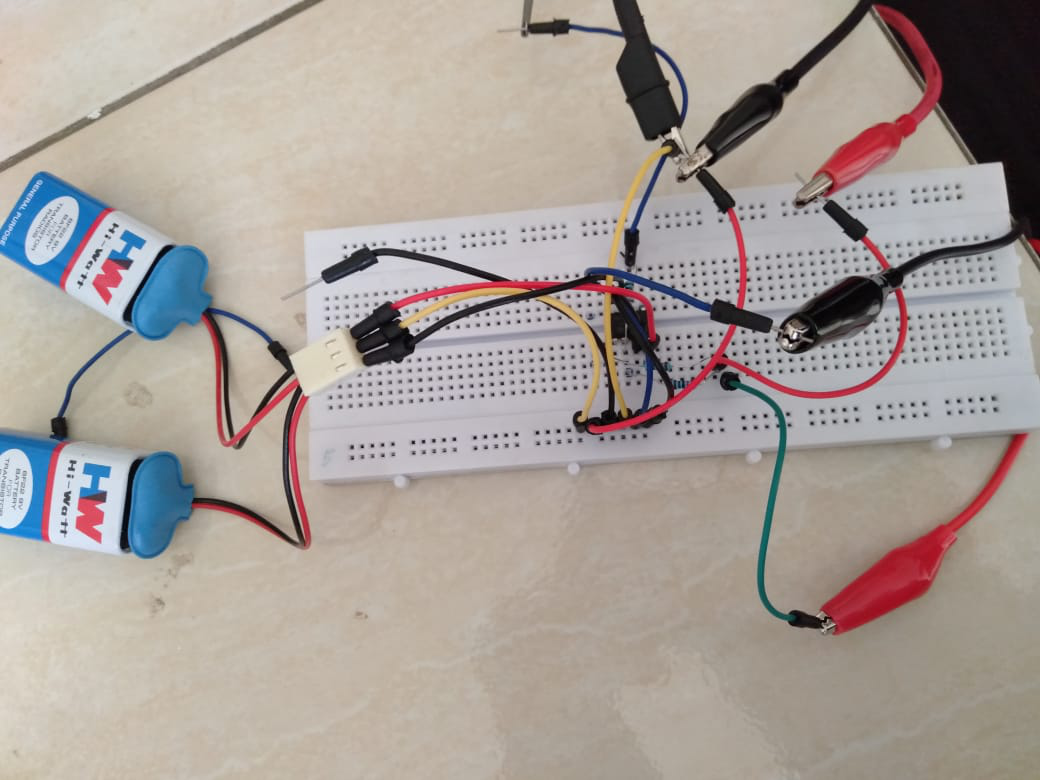
\includegraphics[width=12cm, height=5cm]{Adder1.png}

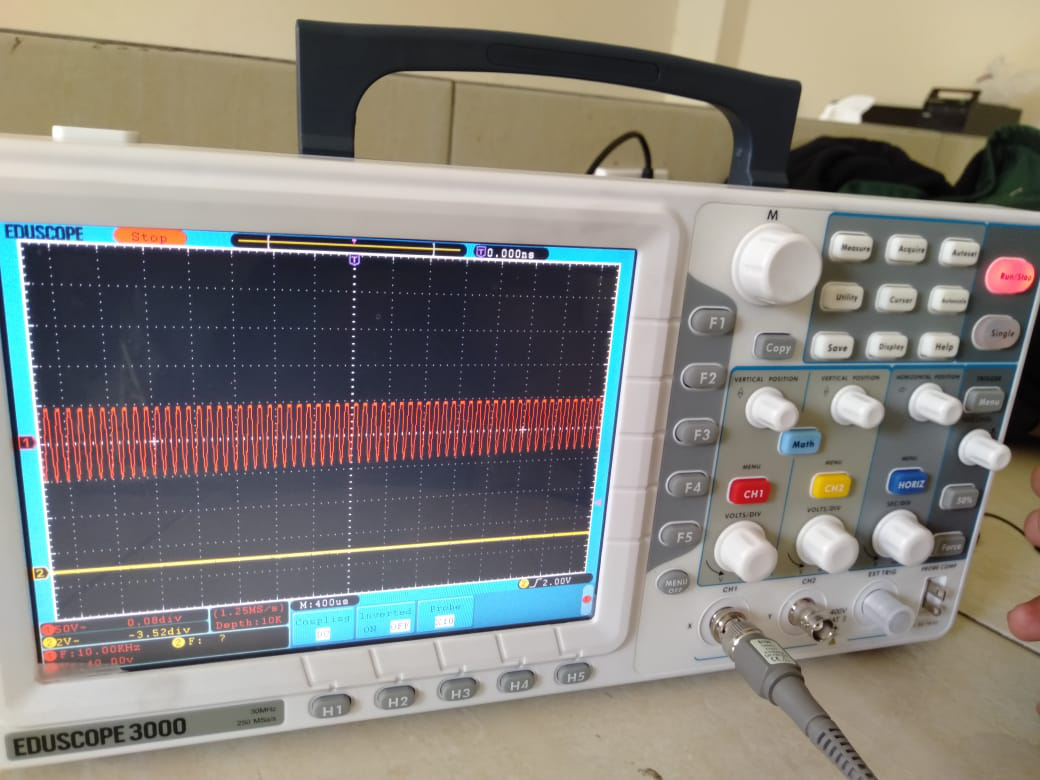
\includegraphics[width=12cm, height=6cm]{Adder2.png}

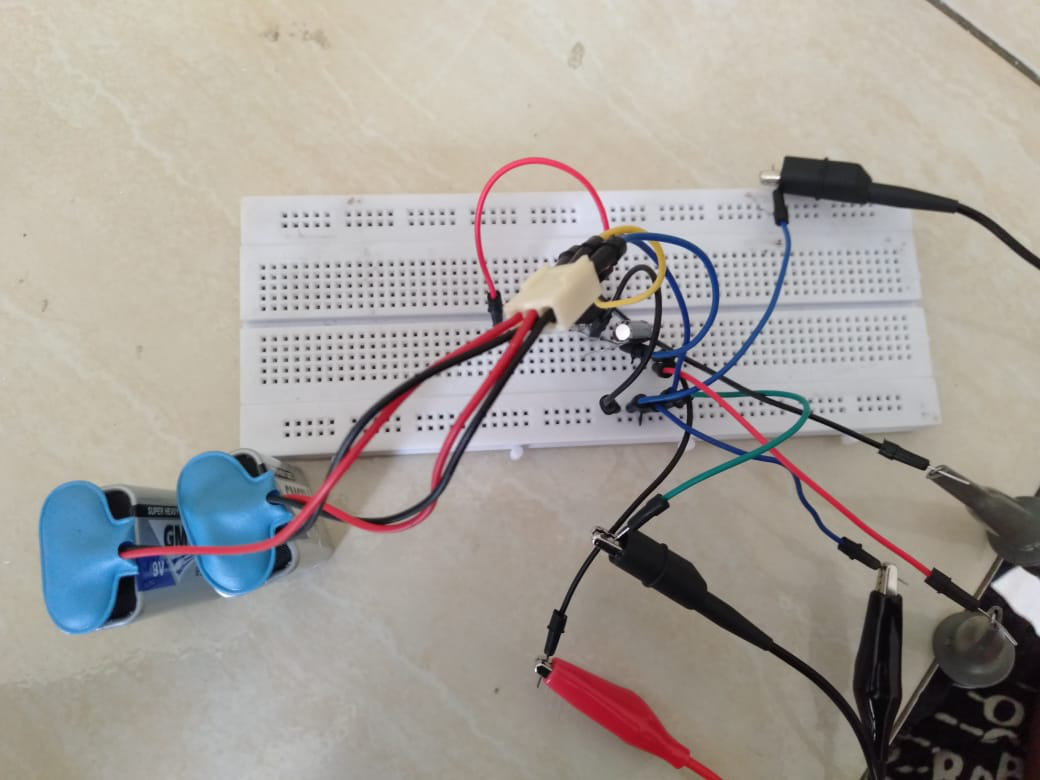
\includegraphics[width=12cm, height=6cm]{Diferent1.png}
\end{center}
\end{figure}
\vspace{2cm}

\newpage
\begin{figure}
\paragraph{Gambar percobaan inverting dan non-inverting}
\paragraph{ }
\begin{center}

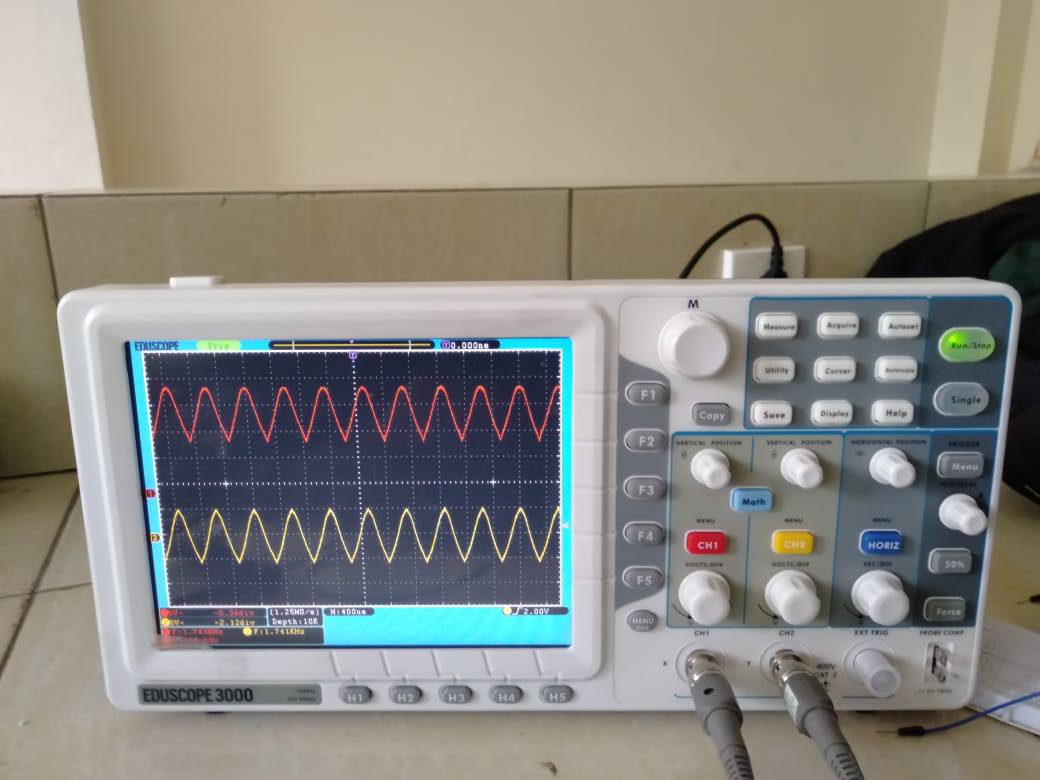
\includegraphics[width=12cm, height=6cm]{Different2.png}

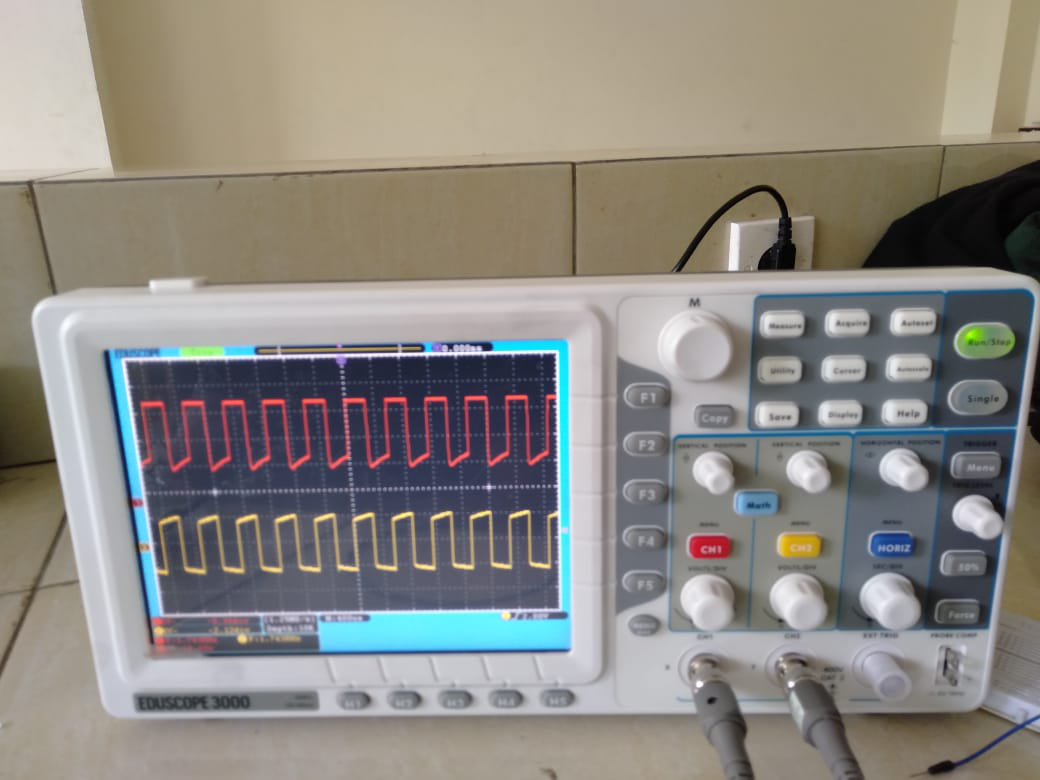
\includegraphics[width=12cm, height=6cm]{Diferent3.png}

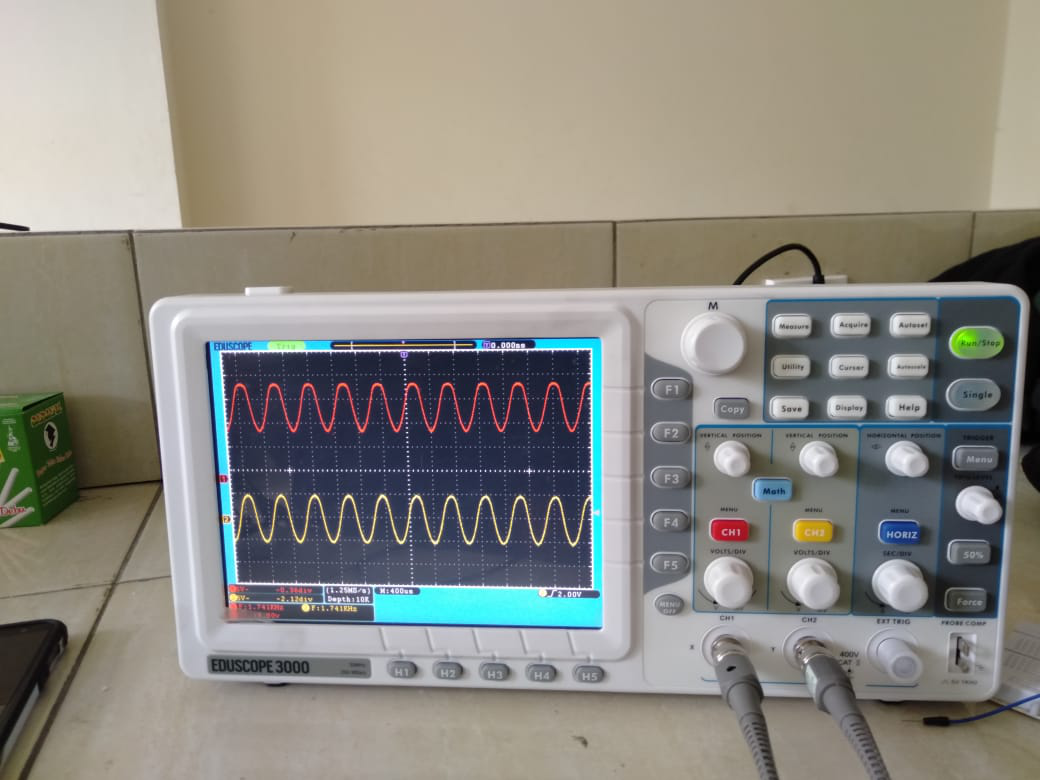
\includegraphics[width=12cm, height=6cm]{Diferent4.png}

\end{center}
\end{figure}
\vspace{2cm}

\newpage
\begin{figure}
\paragraph{Gambar percobaan non-inverting}
\paragraph{ }
\begin{center}

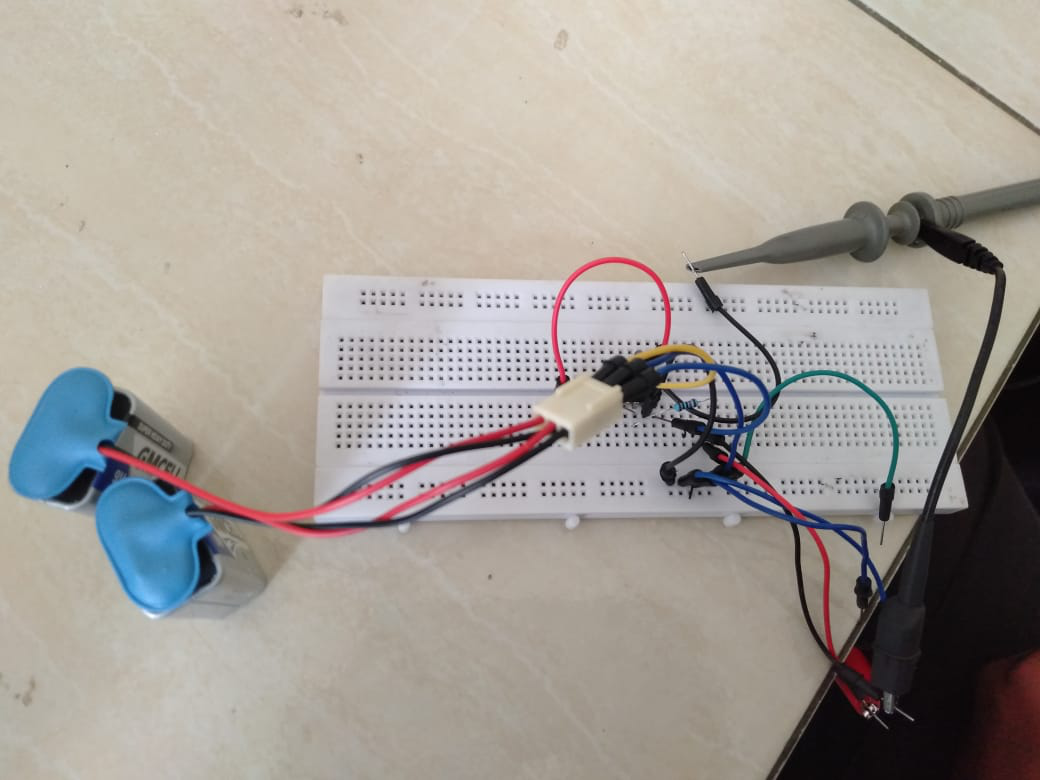
\includegraphics[width=12cm, height=6cm]{Integrator1.png}

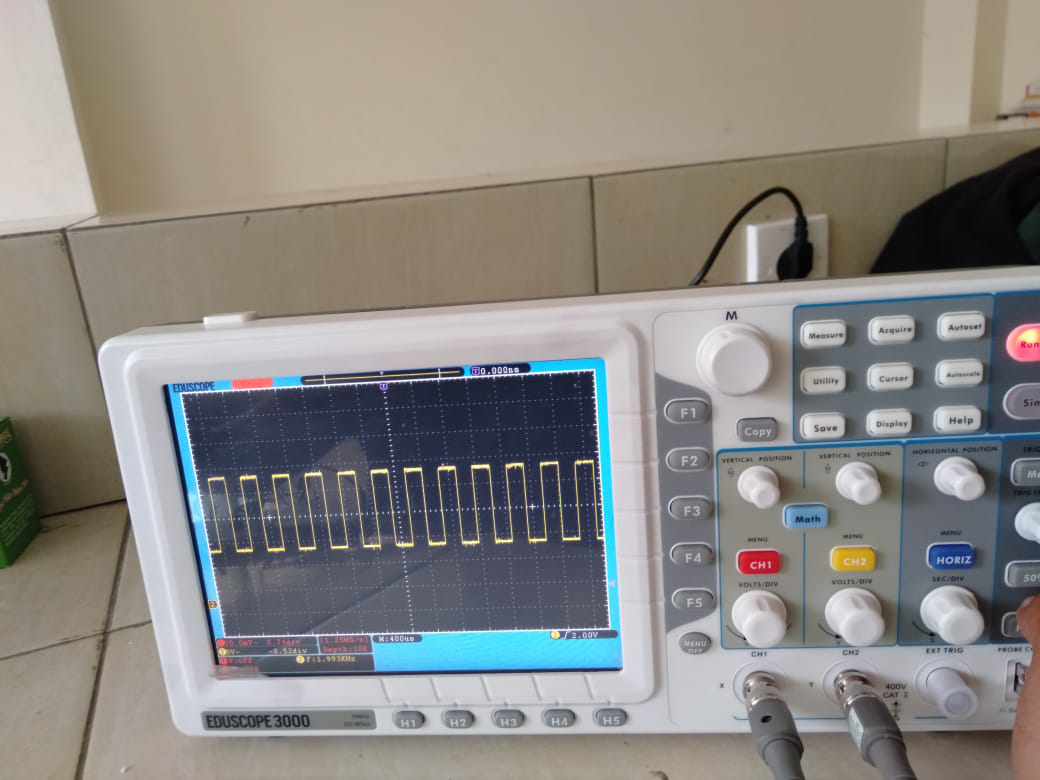
\includegraphics[width=12cm, height=6cm]{Integrator2.png}

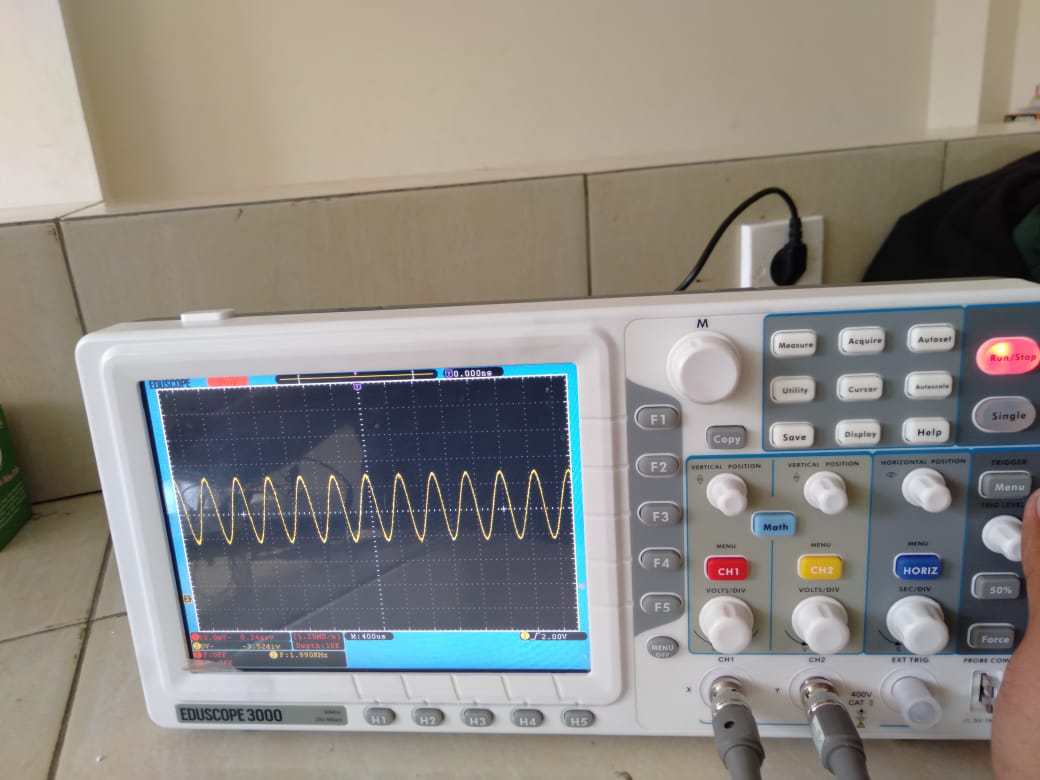
\includegraphics[width=12cm, height=6cm]{Integrator3.png}

\end{center}
\end{figure}
\vspace{2cm}

\newpage
\begin{figure}
\paragraph{Gambar percobaan non-inverting}
\paragraph{ }
\begin{center}

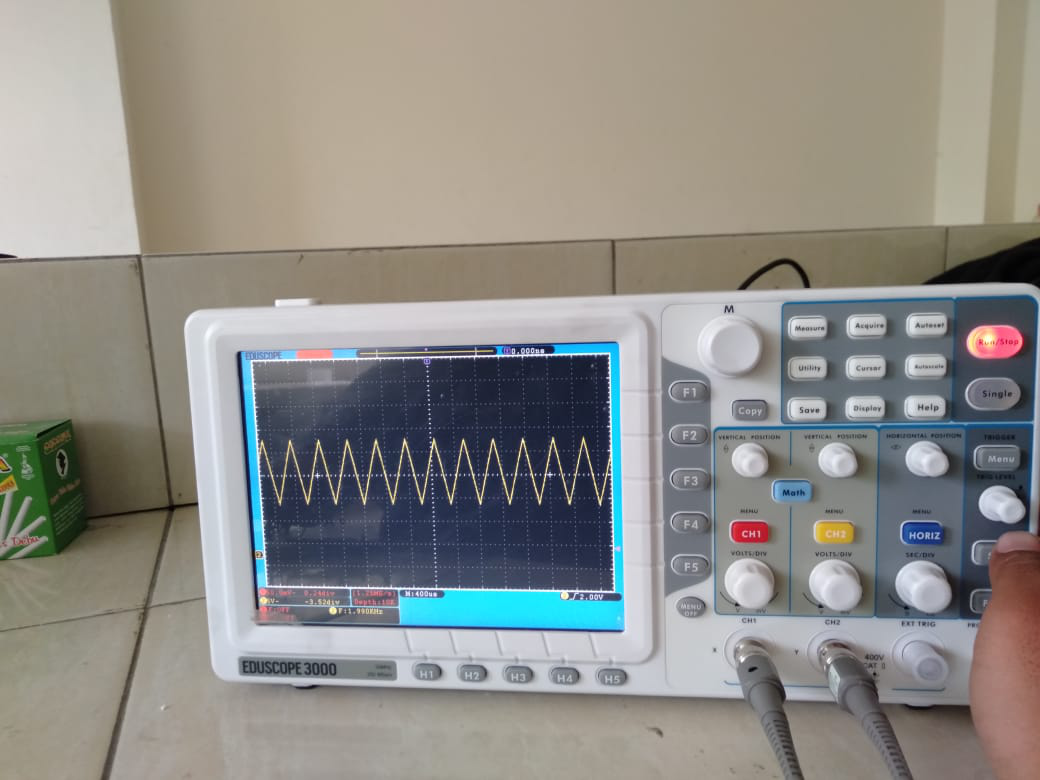
\includegraphics[width=12cm, height=6cm]{Integrator4.png}

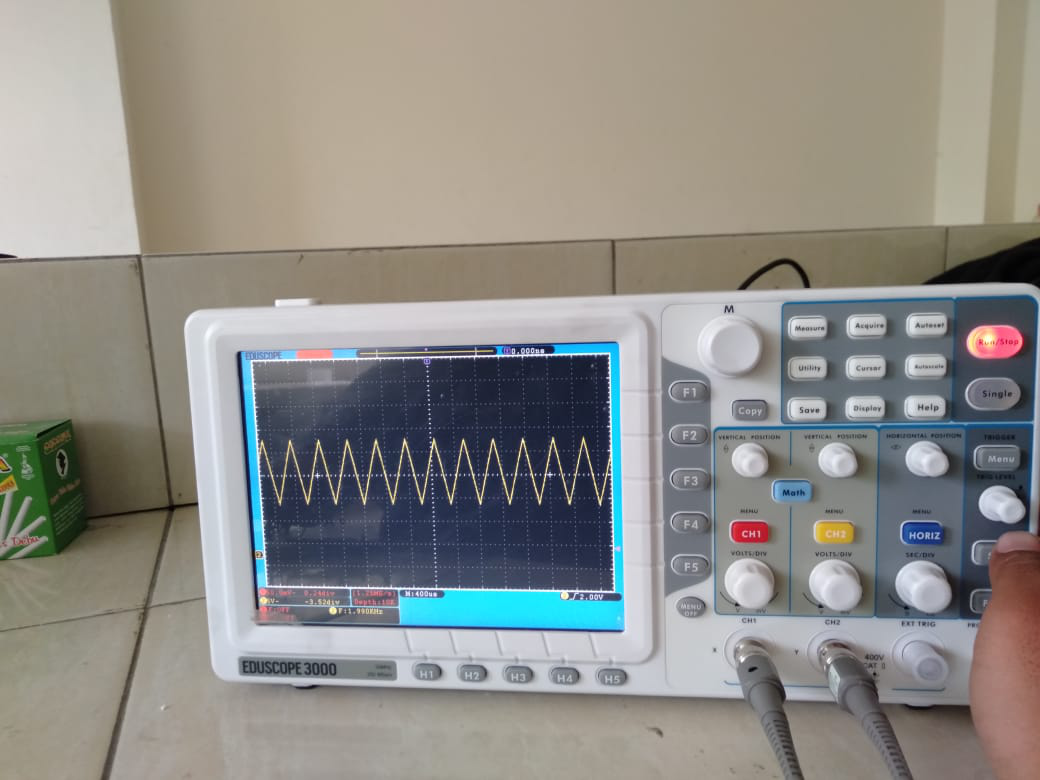
\includegraphics[width=12cm, height=6cm]{Integrator5.png}

\end{center}
\end{figure}
\vspace{2cm}


\end{document} %Penulisan Laporan Berakhir
